\chapter{船岸连接系统结构与分析}

船岸连接(Ship-to-Shore Connection),在不同的文献中有不同的名称,如冷熨烫(Cold Ironing)、岸侧电源(Shore-Side Electricity,SSE)、
岸电供电(Onshore Power Supply,OPS)、船舶岸电系统(Alternative Maritime Power Supplly,AMPS)。
虽然名称有所不同,但它们都涉及到停泊船舶靠港后关闭其船载辅助发动机,并使用港口提供的清洁能源为船载主要系统供电,
满足所有如照明、制冷和货物卸设施等船载设备的电力需求。这种技术允许停泊的船只使用船舶岸电,而不是依靠辅助发动机产生的
电力,从而减少港口污染物的排放。

\section{船岸连接系统的组成}

如图\ref{fig:船岸连接系统示意图}所示,船岸连接系统是由三个基本部分组成:岸侧电力系统和基础设施、电缆管理系统和船侧连接系统。

\begin{figure}[!htp]
	\centering
	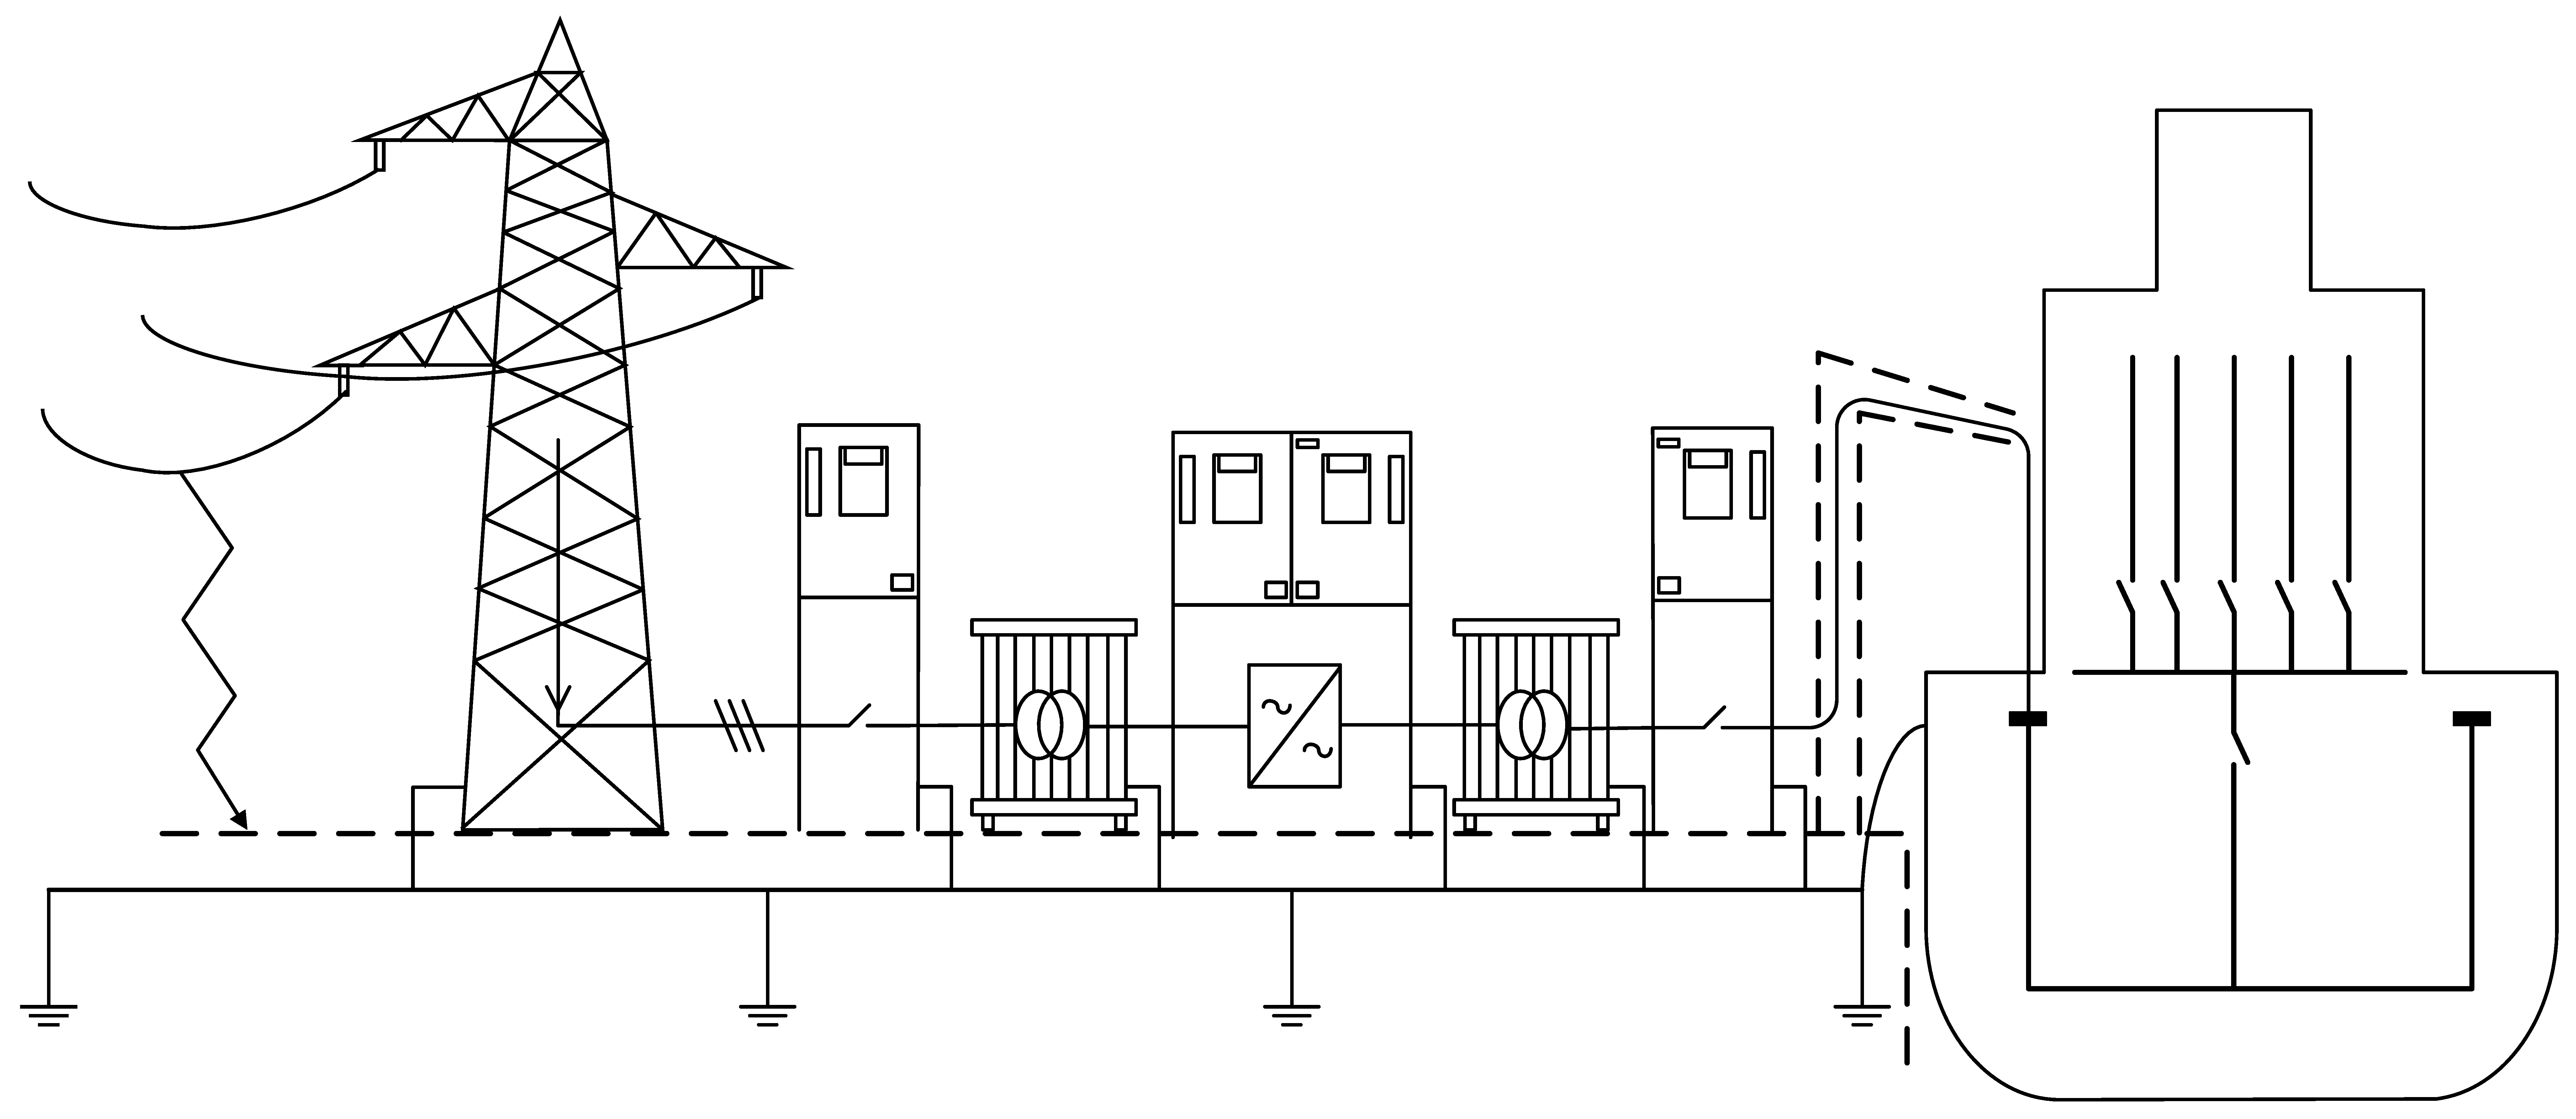
\includegraphics[width=0.95\textwidth]{chapter2/船岸连接系统示意图.pdf}
	\caption{船岸连接系统示意图}
	\label{fig:船岸连接系统示意图}
\end{figure}

岸侧电力系统负责将高压变电站的电力传输到泊位附近的连接点,即终端配电箱,以不间断的方式在船舶电力接收系统之间切换等。首先通过变压器将电网高压转换为低压。
随后,变流系统将对网侧电压变压变频,并通过变压器升至船舶电力系统所需的电压。船岸连接系统应用的电压等级不同,
所需电压由船舶类型决定:一般远洋货轮,大型集装箱船采用高压岸电,小型散货船主要采用低压。电缆管理系统包括连接岸侧连接点、
船载受电设备的电缆和设备。电缆连接设备必须满足电缆的收放功能,与快速连接的能力,不使用时应存放在船上、岸上或者
驳船上。船侧连接系统是在原有的电力系统上增加接受单元,包括电缆绞车、变压器以及相关控制系统等。

\begin{figure}[!htp]
	\centering
	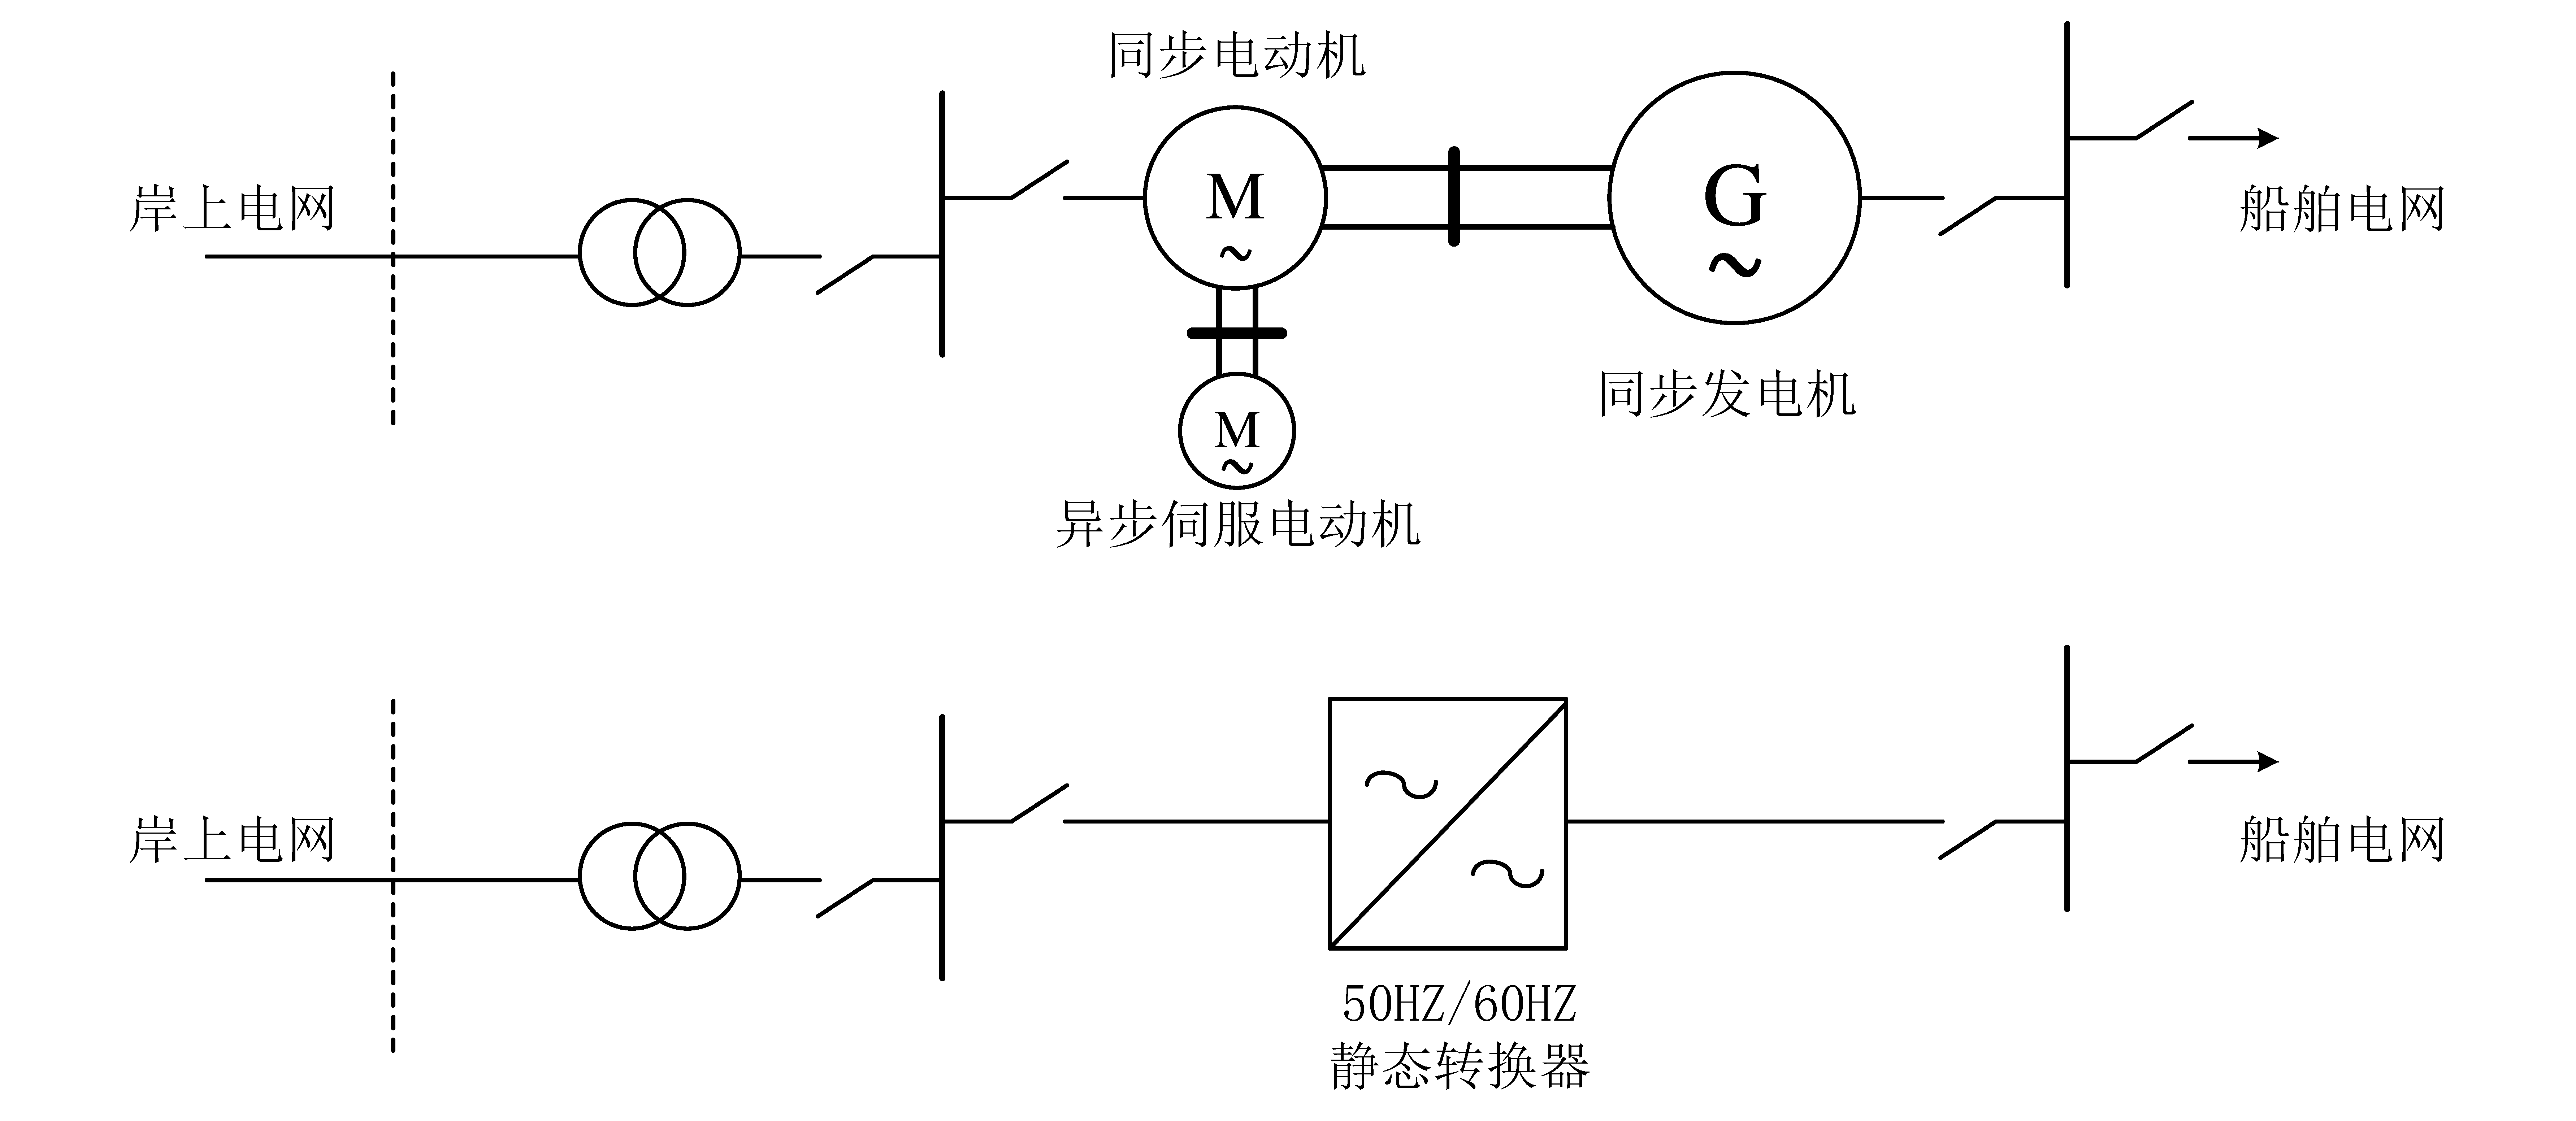
\includegraphics[width=0.85\textwidth]{chapter2/旋转形态转换器对比.pdf}
	\caption{传统旋转变频与静态电源变频对比}
	\label{fig:传统旋转变频与静态电源变频对比}
\end{figure}

\section{船岸连接系统的供电方式}
船载电站的发电机按电压等级可分为
高压和低压。高压船载电站的电压等级包括11 kV、6.6kV(60Hz)和6kV(50Hz),低压船载电站的电压等级包括400V(50Hz)
和440伏(60赫兹)。

岸电供电系统十分重要,出现故障的话将会给船舶造成很大的损失,如果船舶接岸电系统不需要变频的话技术要简单很多,
当港口陆上电网频率与船舶电网频率不一致时,就需要更多的技术支持和保护。

\subsection{船岸连接高压岸电供电系统}

\begin{figure}[!htp]
	\centering
	\includegraphics[width=0.9\textwidth]{chapter2/高压岸电系统.pdf}
	\caption{高压岸电供电系统}
	\label{fig:高压岸电供电系统}
\end{figure}

\subsection{船岸连接低压岸电供电系统}

\begin{figure}[!htp]
	\centering
	\includegraphics[width=0.9\textwidth]{chapter2/低压岸电系统.pdf}
	\caption{低压岸电供电系统}
	\label{fig:低压岸电供电系统}
\end{figure}

\subsection{船岸连接小容量岸电供电系统}

\begin{figure}[!htp]
	\centering
	\includegraphics[width=0.9\textwidth]{chapter2/小容量岸电系统.pdf}
	\caption{小容量岸电供电系统}
	\label{fig:小容量岸电供电系统}
\end{figure}

\subsection{船岸连接不同方案对比}


% \begin{table}[!htp]
% 	\centering
% 	\caption[船用岸电供电方式比较]{船用岸电供电方式比较}
% 	\label{tab:船用岸电供电方式比较latex}
% 	\resizebox{\textwidth}{!}{%
% 	\begin{tabular}{cccc}  
% 	  \toprule
% 	    & 低压岸电/低压船舶     & 高压岸电/低压船舶        & 高压岸电/高压船舶  \\ 
% 	  \midrule
% 	  岸上系统电压/kV & 0.44          & 6~20             & 6.6/11     \\
% 	  船舶配电电压/kV & 0.44          & 0.4              & 6.6/11     \\
% 	  港口电网频率/Hz & 60            & 50               & 60         \\
% 	  船舶用电频率/Hz & 60            & 50               & 60         \\
% 	  岸电接入方式    & 港口提供电缆        & 港口提供电缆           & 船方提供电缆     \\
% 	  船舶改造复杂性   & 较小            & 较复杂,需要船舶上安装降压变压器 & 较小         \\
% 	  供电操作难易度   & 较复杂,需接驳船和多根电缆 & 较容易,仅需一根电缆       & 较容易,仅需少量电缆 \\
% 	  \bottomrule %添加表格底部粗线
% 	\end{tabular}
% 	}
% \end{table}

\begin{table}[!htp]
	\centering
	\caption[船用岸电供电方式比较]{船用岸电供电方式比较}
	\label{tab:船用岸电供电方式比较}
	\resizebox{\textwidth}{!}{%
	\begin{tabular}{c}
		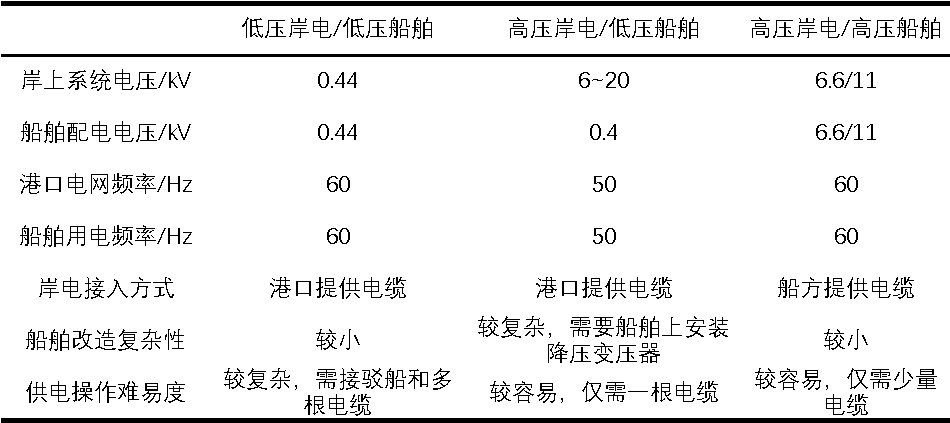
\includegraphics{chapter2/船用岸电供电方式比较.pdf} 
	\end{tabular}
	}
\end{table}

\section{船岸连接系统面临的问题}
\subsection{船舶岸电供电并网切换}
船岸电力的电网连接是在船的柴油发电机和岸上电源之间。并网需要满足四个条件:船舶发电机的相序、幅值、相位、频率
必须与岸电一致。保持相同的相序尤为重要。影响瞬时电压差的三个因素是频率差、相位差和电压差。船岸自动准同步并网
的四个条件如下:
(1)船舶电源的相序必须等于岸上电源的相序;
(2)船舶电源的电压幅值必须等于岸上电源的电压幅值;
(3)船舶电源的频率必须等于岸上电源的频率;
(4)船舶电源的相位必须等于岸上电源的相位。
这些条件在理想情况下得到满足。事实上,相位、频率和振幅不可能同时完全一致。但只要船电和岸电的相位、频率、幅度差
在一定值内,涌流就在系统可接受的范围内,所以可以进行船岸并网。


\cite{SP10}船舶岸电系统具备船电、岸电快速切换连接技术,通过船上同期装置,与岸电电源实现热并网,保证供电安全
可靠。船舶 岸电 系统接到岸电并网指令后,自动并车装置进行相序检测跟踪,在相序一致的情况 下,采集岸电电源及传
播辅机电源的电压、频率和相角差的信息,并计算判断是否满足以下并车条件:辅机与岸电的频率、相序及 电压幅值保持
一致,并且在并车的瞬间保证船舶辅机与岸电电源的输出电压相角同步。之后 完成并车并实现自动无缝负荷转移。根据船舶岸电
系统不同的供电连接方式,将岸电电源与船舶发电机的切换方式主要分为断电方式和无缝切换方式2种。
1)断电方式:当船舶靠港停泊时,需要首先使船舶上所有的用电设备关闭,并使船舶发电机停止工作,然后连接船舶岸电
系统,最后重新启动船舶的用电设备,实现船舶发电机与岸电电源之间的切换;当船舶离港时,按照相反的顺序操作。
2)同步并车方式:也被称为无缝切换方式,切换过程中不需要关闭 船上所有设备。同步并车方式不会影响船舶上用电设备
的正常运行,对船舶上的重要用电设备具有 重 大意义。无缝切换也是船舶岸电连接技术的发展趋势,对于岸电电源的推广
意义重大。船舶岸电自动并车技术需要保证船舶发电机与岸电电源的电压幅值和频率保持一致,并在并车的瞬间保证船舶发
电机与岸电电 源的输出电压相角同步。如果两路电源不同步就进行切换会造成严重的后果。如果在切换时刻一个电源电压波
形在波峰,另外一个位于波谷,切换过程中将会产生很大的冲击电流。虽然切换装置可能能承受该冲击电流,但严重时可能
会导致用电设备和高压静止频率变换器的自动保护装置动作。



\subsubsection{主动并网切换}
\subsubsection{被动并网切换}

\subsection{并网负载转移方式}
\subsection{逆功率处理方案}
\subsubsection{逆功率产生机理}
\subsubsection{逆功率的处理}
\subsubsection{不同控制方案简单对比}




\subsection{岸船连接段系统压降解决方案}

\subsubsection{隔离变压器的压降问题}
\subsubsection{输出电缆的压降问题}


\subsection{三相输出电压平衡控制技术}
\subsection{船岸等电位处理方案}



\section{本章小结}


